\documentclass[a4paper,11pt]{article}
\usepackage{a4wide}
\usepackage{fullpage}
\usepackage[utf8x]{inputenc}

\usepackage[light,math]{anttor}
\usepackage[T1]{fontenc}

%\usepackage[slovene]{babel}
%\selectlanguage{slovene}
\usepackage[toc,page]{appendix}
\usepackage[pdftex]{graphicx} 

\usepackage{lmodern}
\usepackage{amsmath}
\usepackage{amssymb}
\usepackage{amsthm}
\usepackage{amsfonts}
\usepackage{mathtools}
\usepackage{enumitem}
\usepackage{amsfonts}
\usepackage{amsmath}
\usepackage{setspace}
\usepackage{color}
\definecolor{light-gray}{gray}{0.95}
\usepackage{listings} 
\usepackage{hyperref}

\renewcommand{\baselinestretch}{1.2} 
\renewcommand{\appendixpagename}{Priloge}


\title{Machine Learning with Graphs \\
\textbf{CS224W Homework 1} }
\author{Sara Bizjak  |  27202020}
\date{October 2021}

%%%%%%%%%%%%%%%%%%%%%%%%%%%%%%%%%%%%%%%%%%%%%%%%%%%%%%%%%%%%%%%%%%%%%%%%%%%%%%%%%%%%%%%%%%%%%%%%%%%%%%%%%%%%%%%%%%%%%%%%%%%%%%%%%

\begin{document}

\maketitle

%%%%%%%%%%%%%%%%%%%%%%%%%%%%%%%%%%%%%%%%%%%%%%%%%%%%%%%%%%%%%%%%%%%%%%%%%%%%%%%%%%%%%%

\section{Link Analysis}

We have the following users and their teleport sets:
\begin{itemize}
    \item A: \{1, 2, 3\},
    \item B: \{3, 4, 5\},
    \item C: \{1, 4, 5\},
    \item D: \{1\}.
\end{itemize}
Therefore, their teleport vectors can be expressed as:
\begin{itemize}
    \item $t_A = [\frac{1}{3}, \frac{1}{3}, \frac{1}{3}, 0, 0]$
    \item $t_B = [0, 0, \frac{1}{3}, \frac{1}{3}, \frac{1}{3}]$
    \item $t_C = [\frac{1}{3}, 0, 0, \frac{1}{3}, \frac{1}{3}]$
    \item $t_D = [1, 0, 0, 0, 0]$
\end{itemize}
We are computing the personalized PageRank vectors for the following users assuming fixed teleport parameter $\beta$.
\\
Note that from $\beta t_1 + (1 - \beta) t_2 = t_3$ follows $\beta v_1 + (1 - \beta) v_2 = v_3$.

%%%%%%%%%%%%%%%%%%%%%%%%%%%%%%%%%%%%%%%%%%%%%%%%%%%%%%%%%%%%%%%%%%%%%%%%%%%%%%%%%%%%%%
% 1.1 Eloisw, whose interests are represented by the teleport set {2}.
\subsection{Presonalized PrageRank I}

User Eloise, denoted as $E$, with teleport set $\{2\}$ and teleport vector $t_E = [0, 1, 0, 0, 0]$.
\\
We want to express $t_E$ as a linear combination of $t_A, t_B, t_C, t_D$. It follows
\\
\begin{align*}
t_E = [0, 1, 0, 0, 0] = \alpha \cdot \left[\frac{1}{3}, \frac{1}{3}, \frac{1}{3}, 0, 0 \right] 
                        + \beta \cdot \left[0, 0, \frac{1}{3}, \frac{1}{3}, \frac{1}{3}\right]
                        + \gamma \cdot \left[\frac{1}{3}, 0, 0, \frac{1}{3}, \frac{1}{3}\right]
                        + \delta \cdot \left[1, 0, 0, 0, 0\right]
\end{align*}

\begin{align*}
0 &= \frac{1}{3} \alpha  \ \ \ \ \ \ \ + \frac{1}{3} \gamma + \delta
\\
1 &= \frac{1}{3}  \alpha 
\\
0 &= \frac{1}{3} \alpha + \frac{1}{3} \beta 
\\
0 &= \ \ \ \ \ \ \ \ \frac{1}{3} \beta + \frac{1}{3} \gamma 
\\
0 &= \ \ \ \ \ \ \ \ \frac{1}{3} \beta + \frac{1}{3}  \gamma 
\\
&\Rightarrow \alpha = 3, \beta = - 3, \gamma = 3, \delta = -2
\end{align*}
so 
\begin{align*}
t_E = 3 \cdot t_A -3 \cdot t_B + 3 \cdot t_C - 2 \cdot t_D
\end{align*}
and 
\begin{align*}
    v_E = 3 \cdot v_A -3 \cdot v_B + 3 \cdot v_C - 2 \cdot v_D.
\end{align*}

%%%%%%%%%%%%%%%%%%%%%%%%%%%%%%%%%%%%%%%%%%%%%%%%%%%%%%%%%%%%%%%%%%%%%%%%%%%%%%%%%%%%%%
% User Felicity, whose interests are represented by the teleport set {5}.
\subsection{}
User Felicity, denoted as $F$, with teleport set $\{5\}$ and teleport vector $t_F = [0, 0, 0, 0, 1]$.
\\
We want to express $t_F$ as a linear combination of $t_A, t_B, t_C, t_D$. 
\\
Intuitively, it seems impossible to do that, since the last two coordinates of teleport vectors are always present together and have the same values, so we cannot sum $4^{th}$ coordinate to 0 and $5^{th}$ to 1.
Formally,
\begin{align*}
    t_F = [0, 0, 0, 0, 1] = \alpha \cdot \left[\frac{1}{3}, \frac{1}{3}, \frac{1}{3}, 0, 0 \right] 
                            + \beta \cdot \left[0, 0, \frac{1}{3}, \frac{1}{3}, \frac{1}{3}\right]
                            + \gamma \cdot \left[\frac{1}{3}, 0, 0, \frac{1}{3}, \frac{1}{3}\right]
                            + \delta \cdot \left[1, 0, 0, 0, 0\right]
\end{align*}

\begin{align*}
        0 &= \frac{1}{3} \alpha  \ \ \ \ \ \ \ + \frac{1}{3} \gamma + \delta
        \\
        0 &= \frac{1}{3}  \alpha 
        \\
        0 &= \frac{1}{3} \alpha + \frac{1}{3} \beta 
        \\
        0 &= \ \ \ \ \ \ \ \ \frac{1}{3} \beta + \frac{1}{3} \gamma 
        \\
        1 &= \ \ \ \ \ \ \ \ \frac{1}{3} \beta + \frac{1}{3}  \gamma 
        \\
        &\Rightarrow \text{from the last two equations: } 0 = 1 \text{which is contradiction}
\end{align*}
\noindent
Since $t_F$ cannot be written as linear combination of $t_A, t_B, t_C, t_D$, it also follows that $v_F$ cannot be expressed with $v_A, v_B, v_C, v_D$.

%%%%%%%%%%%%%%%%%%%%%%%%%%%%%%%%%%%%%%%%%%%%%%%%%%%%%%%%%%%%%%%%%%%%%%%%%%%%%%%%%%%%%%
% User Felicity, whose interests are represented by the teleport set {5}.
\subsection{}
User Glynnis, denoted as $G$, with teleport set $\{1, 2, 3, 4, 5\}$ and teleport vector $t_G = [0.1, 0.2, 0.3, 0.2, 0.2]$.
\\
We want to express $t_G$ as a linear combination of $t_A, t_B, t_C, t_D$. 
\\
\begin{align*}
    t_G = [0.1, 0.2, 0.3, 0.2, 0.2] = \alpha \cdot \left[\frac{1}{3}, \frac{1}{3}, \frac{1}{3}, 0, 0 \right] 
                            + \beta \cdot \left[0, 0, \frac{1}{3}, \frac{1}{3}, \frac{1}{3}\right]
                            + \gamma \cdot \left[\frac{1}{3}, 0, 0, \frac{1}{3}, \frac{1}{3}\right]
                            + \delta \cdot \left[1, 0, 0, 0, 0\right]
\end{align*}

\begin{align*}
        \frac{1}{10} &= \frac{3}{30} = \frac{10}{30} \alpha  \ \ \ \ \ \ \ \ \  \ + \frac{10}{30} \gamma + \delta
        \\
        \frac{2}{10} &= \frac{6}{30} = \frac{10}{30}  \alpha 
        \\
        \frac{3}{10} &= \frac{9}{30} = \frac{10}{30} \alpha + \frac{10}{30}\beta 
        \\
        \frac{2}{10} &= \frac{6}{30} = \ \ \ \ \ \ \ \ \ \ \frac{10}{30} \beta + \frac{10}{30} \gamma 
        \\
        \frac{2}{10} &= \frac{6}{30} = \ \ \ \ \ \ \ \ \ \ \ \frac{10}{30} \beta + \frac{10}{30}  \gamma 
        \\
        &\Rightarrow \alpha = \frac{6}{10}, \beta = \frac{3}{10}, \gamma = \frac{3}{10}, \delta = - \frac{6}{30}
\end{align*}
so 
\begin{align*}
t_G = \frac{3}{5} \cdot t_A + \frac{3}{10} \cdot t_B + \frac{3}{10} \cdot t_C - \frac{1}{5} \cdot t_D
\end{align*}
and 
\begin{align*}
    v_G = \frac{3}{5} \cdot v_A + \frac{3}{10} \cdot v_B + \frac{3}{10} \cdot v_C - \frac{1}{5} \cdot v_D.
\end{align*}


%%%%%%%%%%%%%%%%%%%%%%%%%%%%%%%%%%%%%%%%%%%%%%%%%%%%%%%%%%%%%%%%%%%%%%%%%%%%%%%%%%%%%%
\subsection{}
Suppose that we have already computed the personalized PageRank vectors (denoted as $V$) of a set of users. Then the set af all personalized PageRank vectors that we can compute from $V$ without accessing the web graph
are all linear combinations of vectors from $V$.


%%%%%%%%%%%%%%%%%%%%%%%%%%%%%%%%%%%%%%%%%%%%%%%%%%%%%%%%%%%%%%%%%%%%%%%%%%%%%%%%%%%%%%
\subsection{}
Here we prove that $r = Ar$ is equivalent to $r = \beta M r + \frac{1 - \beta}{N}1$.
\\
Since $A = \beta M + \frac{1 - \beta}{N}11^T$, it follows
\begin{align*}
r = \beta M r + \frac{1 - \beta}{N}11^T r
\end{align*}
Also,
\begin{align*}
11^T = 
    \begin{pmatrix}
        1 & \ldots & 1 \\
        \vdots & \ddots & \vdots \\
        1 & \ldots & 1 
    \end{pmatrix}
\ \ \text{and} \ \ 
r = 
    \begin{pmatrix}
        v_1
        \\
        \vdots
        \\
        v_N
    \end{pmatrix}
\end{align*}
so 
\begin{align*}
    11^T \cdot r = 
    \begin{pmatrix}
        v_1 + v_2 + \ldots + v_N
        \\
        \vdots
        \\
        v_1 + v_2 + \ldots + v_N
    \end{pmatrix}
\end{align*}
Assuming r is normalized $\left( \sum_{i = 1}^{N} r_i = 1 \right)$, it follows
\begin{align*}
    11^T r = 
    \begin{pmatrix}
        1
        \\
        \vdots
        \\
        1
    \end{pmatrix}
\end{align*}
and
\begin{align*}
    r &= Ar 
    \\
    &= \beta M r + \frac{1 - \beta}{N}11^T r
    \\
    &= \beta M r + \frac{1 - \beta}{N} 1
\end{align*}
thus the condition is proved.

%%%%%%%%%%%%%%%%%%%%%%%%%%%%%%%%%%%%%%%%%%%%%%%%%%%%%%%%%%%%%%%%%%%%%%%%%%%%%%%%%%%%%%
%%%%%%%%%%%%%%%%%%%%%%%%%%%%%%%%%%%%%%%%%%%%%%%%%%%%%%%%%%%%%%%%%%%%%%%%%%%%%%%%%%%%%%
%%%%%%%%%%%%%%%%%%%%%%%%%%%%%%%%%%%%%%%%%%%%%%%%%%%%%%%%%%%%%%%%%%%%%%%%%%%%%%%%%%%%%%

\section{Relational Classification I}
After the first iteration:
\begin{itemize}
    \item $P(Y_1 = +) = \frac{1}{2} (\frac{1}{2} + \frac{1}{2}) = \frac{1}{2}$
    \item $P(Y_2 = +) = \frac{1}{4} (\frac{1}{2} + \frac{1}{2} + \frac{1}{2} + 0) = \frac{3}{8}$
    \item $P(Y_3 = +) = \frac{1}{3} (\frac{1}{2} + \frac{3}{8} + 1) = \frac{5}{8}$
    \item $P(Y_4 = +) = \frac{1}{4} (\frac{3}{8} + 0 + \frac{1}{2} + 1) = \frac{15}{32}$
    \item $P(Y_8 = +) = \frac{1}{2} (\frac{15}{32} + \frac{1}{2}) = \frac{31}{64}$
    \item $P(Y_9 = +) = \frac{1}{2} (\frac{31}{64} + 0) = \frac{31}{128}$
\end{itemize}
After the second iteration:
\begin{itemize}
    \item $P(Y_1 = +) = \frac{1}{2} (\frac{3}{8} + \frac{5}{8}) = \frac{1}{2} = 0.5$
    \item $P(Y_2 = +) = \frac{1}{4} (\frac{1}{2} + \frac{5}{8} + \frac{15}{32} + 0) = \frac{51}{128} = 0.4$
    \item $P(Y_3 = +) = \frac{1}{3} (\frac{1}{2} + \frac{51}{128} + 1) = \frac{81}{128} = 0.63$
    \item $P(Y_4 = +) = \frac{1}{4} (\frac{51}{128} + 0 + \frac{31}{64} + 1) = \frac{241}{512} = 0.47$
    \item $P(Y_8 = +) = \frac{1}{2} (\frac{241}{512} + \frac{31}{128}) = \frac{365}{1024} = 0.36$
    \item $P(Y_9 = +) = \frac{1}{2} (\frac{365}{1024} + 0) = \frac{365}{2048} = 0.18$
\end{itemize}

\subsection{}
$P(Y_3 = +) = \frac{81}{128} = 0.63$

\subsection{}
$P(Y_4 = +) =  \frac{241}{512} = 0.47$

\subsection{}
$P(Y_8 = +) = \frac{365}{1024} = 0.36$

\subsection{}
Nodes that belong to class "-" after the second iteration are:
\\
1,2,4,5,8,9.


%%%%%%%%%%%%%%%%%%%%%%%%%%%%%%%%%%%%%%%%%%%%%%%%%%%%%%%%%%%%%%%%%%%%%%%%%%%%%%%%%%%%%%
%%%%%%%%%%%%%%%%%%%%%%%%%%%%%%%%%%%%%%%%%%%%%%%%%%%%%%%%%%%%%%%%%%%%%%%%%%%%%%%%%%%%%%
%%%%%%%%%%%%%%%%%%%%%%%%%%%%%%%%%%%%%%%%%%%%%%%%%%%%%%%%%%%%%%%%%%%%%%%%%%%%%%%%%%%%%%

\section{Relation Classification II}

\subsection{Bootstrap Phase}

\begin{figure}[ht!]
    \centering
    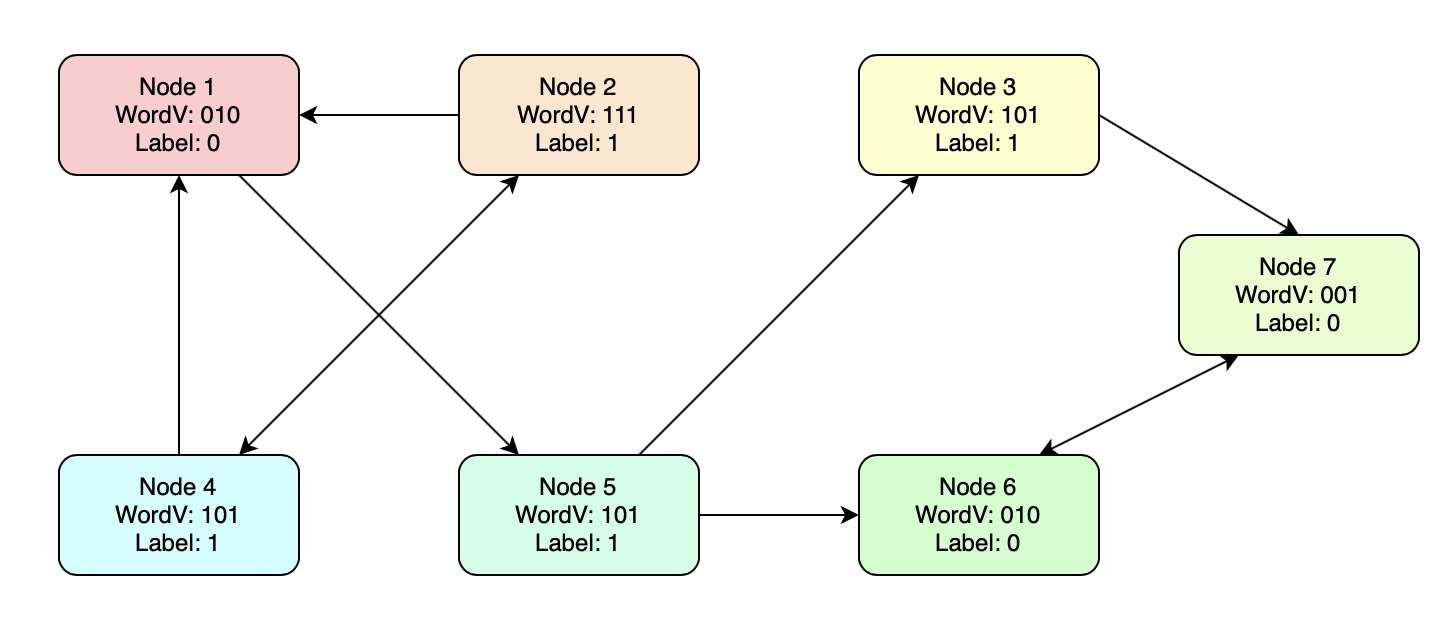
\includegraphics[width=130mm]{Figures/3_1.png}
    \caption{Condition after bootstrap phase.}
\end{figure}

\newpage
\subsection{Iteration 1}

\begin{figure}[ht!]
    \centering
    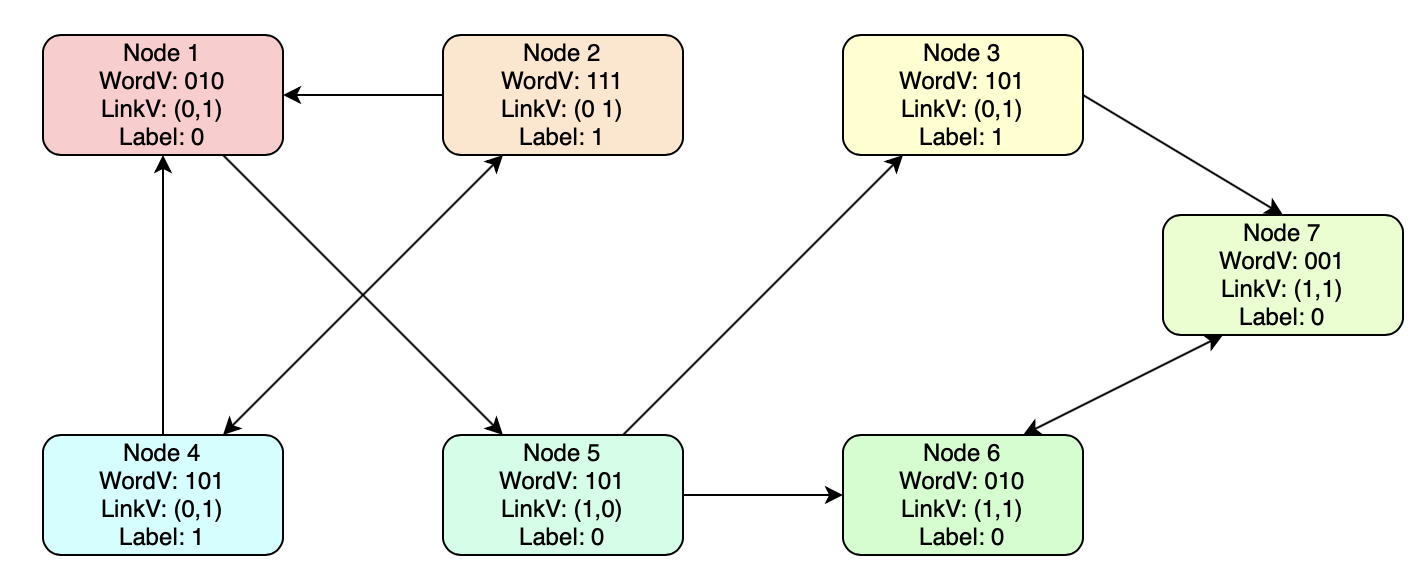
\includegraphics[width=130mm]{Figures/3_2.png}
    \caption{Condition after first iteration.}
\end{figure}

\subsection{Iteration 2}

\begin{figure}[ht!]
    \centering
    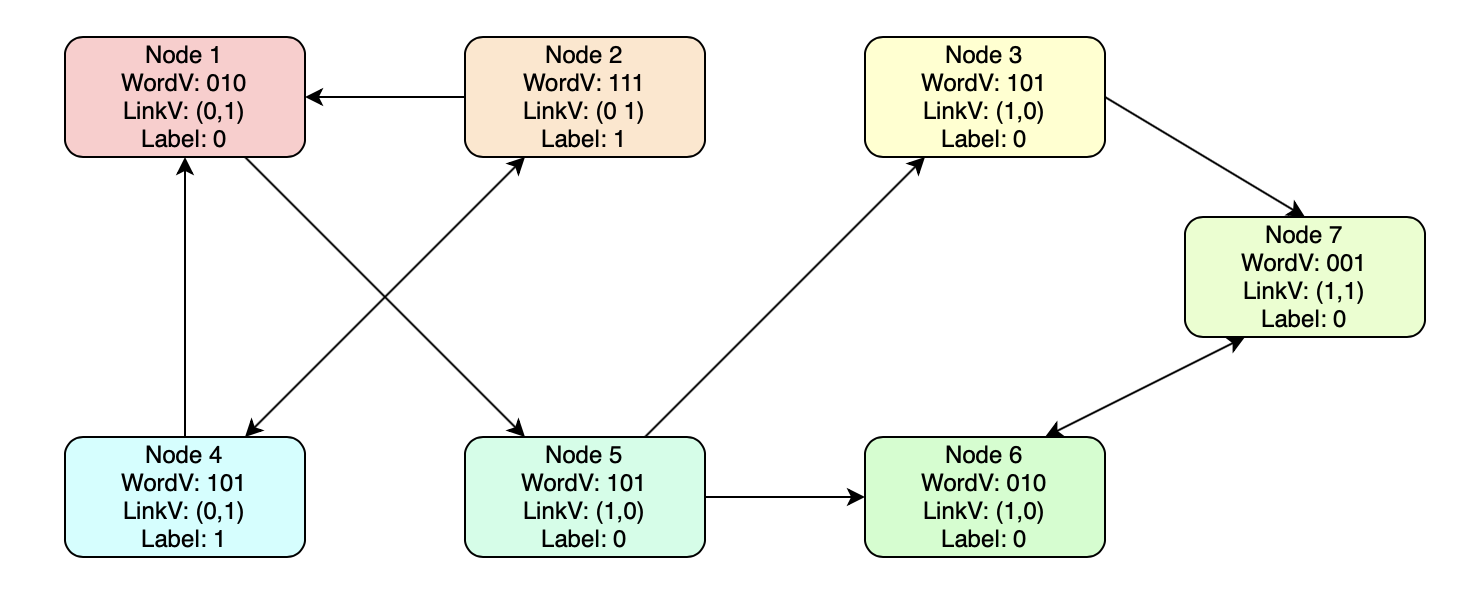
\includegraphics[width=130mm]{Figures/3_3.png}
    \caption{Condition after second iteration.}
\end{figure}

\subsection{Convergence}

If we do one more iteration, all the labels remain the same, so the algorithm converges after three iterations.

%%%%%%%%%%%%%%%%%%%%%%%%%%%%%%%%%%%%%%%%%%%%%%%%%%%%%%%%%%%%%%%%%%%%%%%%%%%%%%%%%%%%%%
%%%%%%%%%%%%%%%%%%%%%%%%%%%%%%%%%%%%%%%%%%%%%%%%%%%%%%%%%%%%%%%%%%%%%%%%%%%%%%%%%%%%%%
%%%%%%%%%%%%%%%%%%%%%%%%%%%%%%%%%%%%%%%%%%%%%%%%%%%%%%%%%%%%%%%%%%%%%%%%%%%%%%%%%%%%%%

\newpage
\section{GNN Expressiveness}

\subsection{Effect of Depth on Expressiveness}

\begin{figure}[ht!]
    \centering
    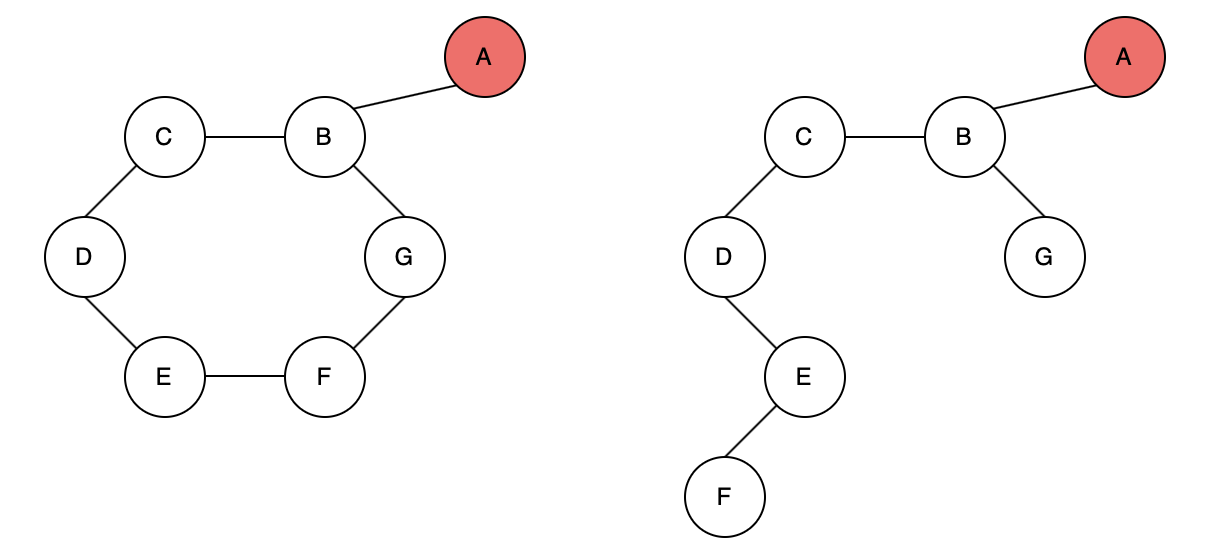
\includegraphics[width=130mm]{Figures/4_1_graph.png}
    \caption{The two given graphs with denoted nodes.}
\end{figure}
\noindent
We now run the GNN to compute node embeddings for the two red nodes.

\begin{figure}[ht!]
    \centering
    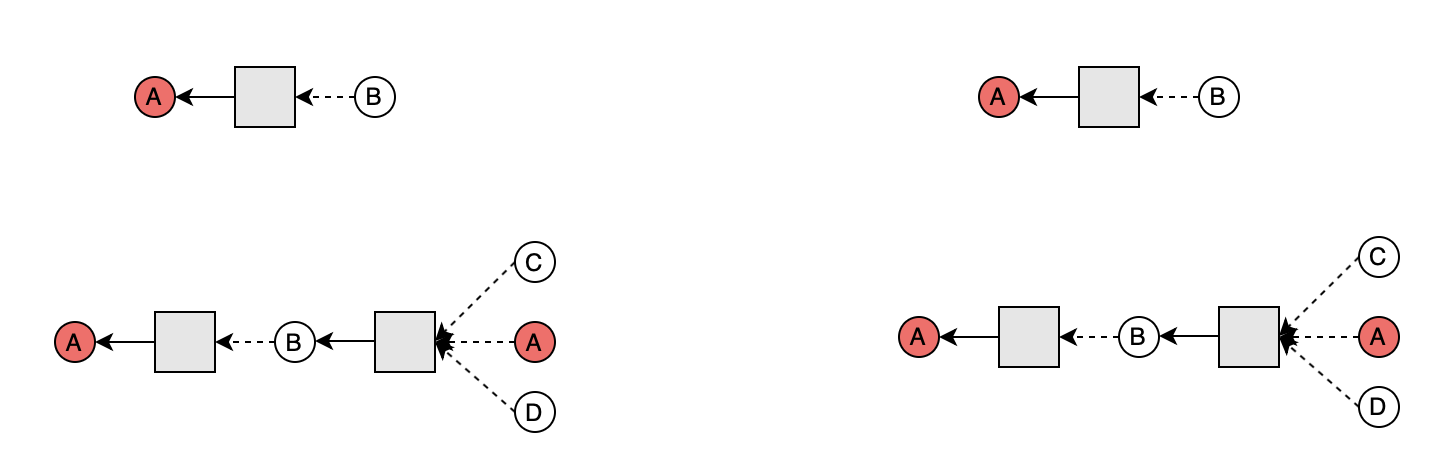
\includegraphics[width=130mm]{Figures/4_1_1and2layer.png}
    \caption{Node embeddings for the red node after first and second layer of message passing are the same, the two red nodes are not distinguished yet.}
\end{figure}

\begin{figure}[ht!]
    \centering
    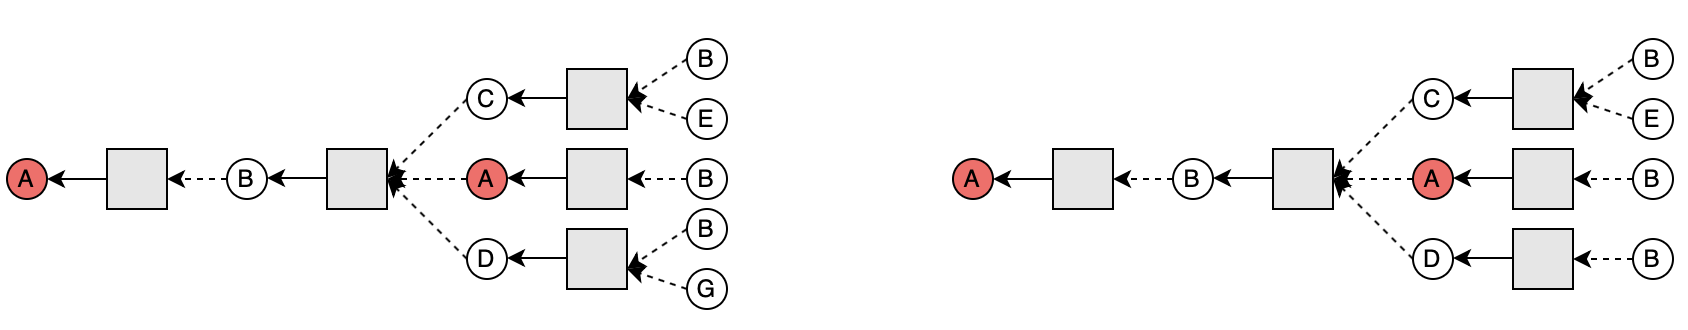
\includegraphics[width=130mm]{Figures/4_1_3layer.png}
    \caption{After third layer of message passing, the red nodes are distinguished, since having different GNN embeddings.}
\end{figure}
\noindent
To conclude, three layers of message passing are needed so that the red two nodes can be distinguished (i.~e., have different GNN embeddings).

%%%%%%%%%%%%%%%%%%%%%%%%%%%%%%%%%%%%%%%%%%%%%%%%%%%%%%%%%%%%%%%%%%%%%%%%%%%%%%%%%%%%%%

\subsection{Random Walk Matrix}

\begin{itemize}
    \item[i] Assume that the current distribution is $r = \{0, 0, 1, 0\}$ and after the random walk, the distribution is $M \times r$. The transition matrix M, where each row of $M$ corresponds with the node id in the graph, is then
            \begin{align*}
                M = 
                \begin{pmatrix}
                    0 & \frac{1}{2} & 0 & \frac{1}{3} \\
                    \frac{1}{2} & 0 & 0 & \frac{1}{3} \\
                    0 & 0 & 0 & \frac{1}{3} \\
                    \frac{1}{2} & \frac{1}{2} & 1 & 0
                \end{pmatrix}    
            \end{align*} 
    \item[ii] Calculation of limiting distribution $r = [\alpha, \beta, \gamma, \delta]^T$, where $\alpha + \beta + \gamma + \delta = 1$ is
            \begin{align*} 
                \begin{pmatrix}
                    \alpha \\
                    \beta \\
                    \gamma \\
                    \delta
                \end{pmatrix} 
                &=
                \begin{pmatrix}
                    0 & \frac{1}{2} & 0 & \frac{1}{3} \\
                    \frac{1}{2} & 0 & 0 & \frac{1}{3} \\
                    0 & 0 & 0 & \frac{1}{3} \\
                    \frac{1}{2} & \frac{1}{2} & 1 & 0
                \end{pmatrix} 
                \times 
                \begin{pmatrix}
                    \alpha \\
                    \beta \\
                    \gamma \\
                    \delta
                \end{pmatrix} 
                \\
                \\
                \begin{pmatrix}
                    \alpha \\
                    \beta \\
                    \gamma \\
                    \delta
                \end{pmatrix} 
                &=
                \begin{pmatrix}
                    \frac{1}{2} \beta + \frac{1}{3} \delta \\
                    \frac{1}{2} \alpha + \frac{1}{3} \delta \\
                    \frac{1}{3} \delta \\
                    \frac{1}{2} \alpha + \frac{1}{2} \beta + \gamma
                \end{pmatrix} 
            \end{align*}
            \begin{align*}
                \text{first + second + third row: } \Rightarrow \alpha &= \frac{1}{2} \beta + \gamma
                \\
                \beta &= \frac{1}{2} \alpha + \gamma
                \ \ \Rightarrow \beta = \alpha
                \\[0.3 cm]
                \Rightarrow = \gamma &= \frac{1}{2} \alpha 
                \\[0.3 cm]
                \Rightarrow \delta &= \frac{3}{2} \alpha
            \end{align*}
            following
            \begin{align*} 
                1 &= \alpha + \beta + \gamma + \delta 
                \\
                1 &= \alpha + \alpha + \frac{1}{2} \alpha + \frac{3}{2} \alpha = 4 \alpha \ \ \Rightarrow \alpha = \frac{1}{4} = 0.25
                \\
                \Rightarrow \beta &= \frac{1}{4} = 0.25, \gamma = \frac{1}{8} = 0.125, \delta = \frac{3}{8} = 0.375
            \end{align*}
            thus the rounded limiting distribution equals
            \begin{align*} 
                r = (0.25, 0.25, 0.13, 0.38)
            \end{align*}
\end{itemize}

%%%%%%%%%%%%%%%%%%%%%%%%%%%%%%%%%%%%%%%%%%%%%%%%%%%%%%%%%%%%%%%%%%%%%%%%%%%%%%%%%%%%%%

\subsection{Relation to Random Walk (i)}

The transition matrix of the random walk is 
$$P = D^{-1} \cdot A.$$

%%%%%%%%%%%%%%%%%%%%%%%%%%%%%%%%%%%%%%%%%%%%%%%%%%%%%%%%%%%%%%%%%%%%%%%%%%%%%%%%%%%%%%

\subsection{Relation to Random Walk (ii)}

If we add a skip connection in aggregation from Q4.3, the new corresponding transition matrix is 
$$P = \frac{1}{2} \cdot I + \frac{1}{2} \cdot D^{-1} \cdot A.$$

%%%%%%%%%%%%%%%%%%%%%%%%%%%%%%%%%%%%%%%%%%%%%%%%%%%%%%%%%%%%%%%%%%%%%%%%%%%%%%%%%%%%%%

\subsection{Over-Smoothing Effect}

We want to prove that Markov chain is aperiodic and irreducible.
\begin{itemize}
    \item \textit{Markov Chain is irreducible.}  Since the graph is connected, we can move around the graph arbitrarily, meaning that from every node we can get to every other.
    \item \textit{Markov chain is aperiodic.}  It follows from the fact that the graph has no bipartite components.
\end{itemize}
Then, by the Markov Convergence Theorem, the node embedding $h_i^{(l)}$ will converge as $l \rightarrow \infty$, more precisely, it will converge to $h_i$ for node $i$.
%%%%%%%%%%%%%%%%%%%%%%%%%%%%%%%%%%%%%%%%%%%%%%%%%%%%%%%%%%%%%%%%%%%%%%%%%%%%%%%%%%%%%%

\subsection{Learning BFS with GNN}

Update rule for the $i$-th node for the GNN can be written as
$$
h_i^{(l + 1)} = \max_{j \in N_i} \left( h_i^{(l)}, h_j^{(l)} \right)
$$


%%%%%%%%%%%%%%%%%%%%%%%%%%%%%%%%%%%%%%%%%%%%%%%%%%%%%%%%%%%%%%%%%%%%%%%%%%%%%%%%%%%%%%%%%%%%%%%%%%%%%%%%%%%%%%%%%%%%%%%%%%%%%%%%%%%%%%%%%%%%%%%%%%%%%%%%%%%%%%%%%%%%%%%%%%%%
%%%%%%%%%%%%%%%%%%%%%%%%%%%%%%%%%%%%%%%%%%%%%%%%%%%%%%%%%%%%%%%%%%%%%%%%%%%%%%%%%%%%%%%%%%%%%%%%%%%%%%%%%%%%%%%%%%%%%%%%%%%%%%%%%%%%%%%%%%%%%%%%%%%%%%%%%%%%%%%%%%%%%%%%%%%%

\section{Node Embedding and its relation to matrix factorization}

\subsection{Simple matrix factorization}

The decoder here is the dot product
$$
z_i ^ T \cdot z_j
$$

%%%%%%%%%%%%%%%%%%%%%%%%%%%%%%%%%%%%%%%%%%%%%%%%%%%%%%%%%%%%%%%%%%%%%%%%%%%%%%%%%%%%%%

\subsection{Alternate matrix factorization}

The objective function for the corresponding matrix factorization would be 
$$
\min_{Z, W} || A - Z^TWZ ||_2
$$

%%%%%%%%%%%%%%%%%%%%%%%%%%%%%%%%%%%%%%%%%%%%%%%%%%%%%%%%%%%%%%%%%%%%%%%%%%%%%%%%%%%%%%

\subsection{Relation to eigendecomposition}

The matrix $W$ has to be diagonal. The values on its diagonal would be eigen values and matrix $Z$ would have eigen vectors in its columns.

%%%%%%%%%%%%%%%%%%%%%%%%%%%%%%%%%%%%%%%%%%%%%%%%%%%%%%%%%%%%%%%%%%%%%%%%%%%%%%%%%%%%%%

\subsection{Multi-hop node similarity}

We know that in the $(u, v)$-th place in matrix $A^k$ is the number of different paths of length $k$ between nodes $u$ and $v$. 
So if we look at elements of the matrix 
$$
A_p = \sum_{i = 1}^k A^i
$$
we will get the number of paths of length at most $k$ between any of the two nodes in a graph.
However, if two nodes are silimar when connected by at least one path of length at most $k$, we do not need to count how many such paths exist, 
but it is enough to construct a "classification" matrix, just using 0 and 1 to denote wether there exist a path of length at most $k$ or not. Let us denote such matrix with $A_{opt}$.
Therefore, we are solving the matrix factorization problem for matrix $A_{opt}$ instead of $A_p$ (I guess even with $A_p$ would be possible, but $A_{opt}$ is optimized).
So,
$$
\min_Z || A_{opt} - Z^T Z ||_2
$$


%We are interested in paths of length at most $k$ between two nodes, so we need to sum up over all number of paths from $1$ to $k$, i.~e.~ $\sum_{i = 1}^k A_{(u, v)}^i$,
%so we are solving the matrix factorization problem for matrix $A^{(u, v)} = \sum_{i = 1}^k A_{(u, v)}^i$:
%$$
%\min_Z || A^{(u, v)} - Z^T Z ||_2
%$$

%%%%%%%%%%%%%%%%%%%%%%%%%%%%%%%%%%%%%%%%%%%%%%%%%%%%%%%%%%%%%%%%%%%%%%%%%%%%%%%%%%%%%%

\subsection{Limitation of node2vec (i)}

On the figure below, we have two cliques and a "bridge/path" between them. 
On each clique, all nodes are connected and will, therefore, have similar embedding (a node from left clique will have similar embeding than other nodes in left clique and similar for the right one).
However, if we are moving around left clique on the graph, there will be a very small probability that our random walk will lead us to reach the right clique. 
To sum up, even if the strusture of the left and right clique is the same, the nodes on the left cliques will have different (= not similar) embeddings than the nodes on the right clique.

\begin{figure}[ht!]
    \centering
    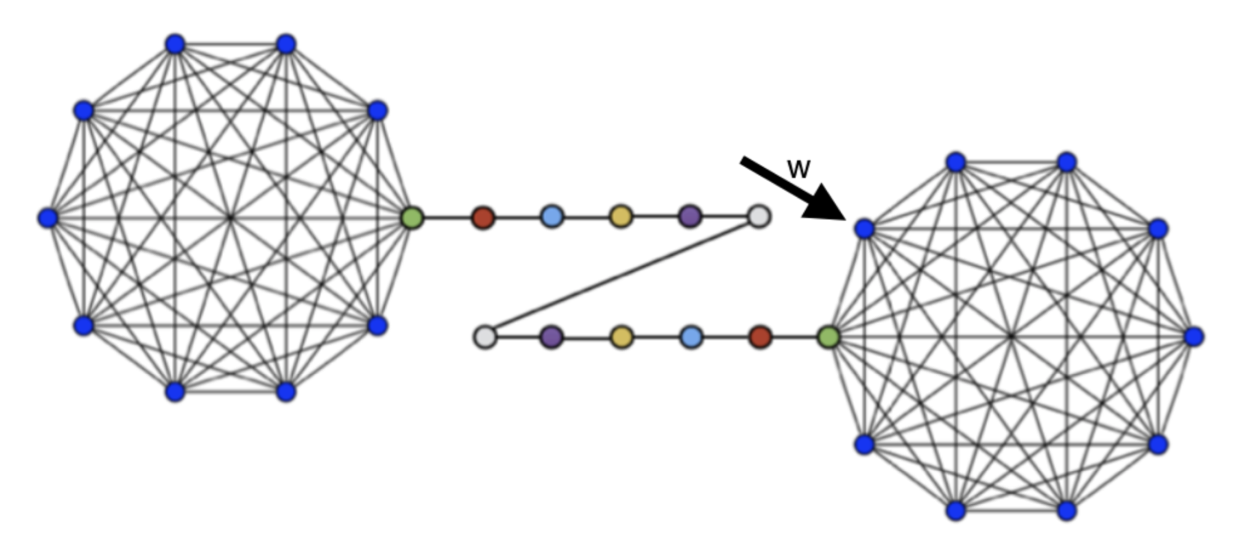
\includegraphics[width=130mm]{Figures/5_5.png}
    \caption{Given graph.} 
\end{figure}

\subsection{Limitation of node2vec (ii)}

Assume we are at a position of node $w$ in the graph on the figure above. Taking one step further with 
\texttt{node2vec} algorithm, we can only reach the neighbors, that is, nodes in the same clique in which $w$ belongs (right one), however, with \texttt{struct2vec} algorithm we can reach all nodes, since all nodes are connected.

%%%%%%%%%%%%%%%%%%%%%%%%%%%%%%%%%%%%%%%%%%%%%%%%%%%%%%%%%%%%%%%%%%%%%%%%%%%%%%%%%%%%%%

\subsection{Limitation of node2vec (iii)}

To consider different $g_k$'s during the random walk means that we change the distance $k$. 
With changing $k$ we can get a better approximation of the graph 
and a better insight on which nodes are similar.



%%%%%%%%%%%%%%%%%%%%%%%%%%%%%%%%%%%%%%%%%%%%%%%%%%%%%%%%%%%%%%%%%%%%%%%%%%%%%%%%%%%%%%

\subsection{Limitation of node2vec (iv)}

In contrast to the \texttt{node2vec}, with \texttt{struct2vec} the nodes in both two cliques will have similar embeddings, since here we can reach all nodes, not only neighbors, so the random walk has more probability to go from one clique to another.
Even more, since the algorithm captures the similarity in the structure between nodes, the nodes with the same colors will have similar embeddings.

%%%%%%%%%%%%%%%%%%%%%%%%%%%%%%%%%%%%%%%%%%%%%%%%%%%%%%%%%%%%%%%%%%%%%%%%%%%%%%%%%%%%%%%%%%%%%%%%%%%%%%%%%%%%%%%%%%%%%%%%%%%%%%%%%%%%%%%%%%%%%%%%%%%%%%%%%%%%%%%%%%%%%%%%%%%%
%%%%%%%%%%%%%%%%%%%%%%%%%%%%%%%%%%%%%%%%%%%%%%%%%%%%%%%%%%%%%%%%%%%%%%%%%%%%%%%%%%%%%%%%%%%%%%%%%%%%%%%%%%%%%%%%%%%%%%%%%%%%%%%%%%%%%%%%%%%%%%%%%%%%%%%%%%%%%%%%%%%%%%%%%%%%


\begin{thebibliography}{99}
    \bibitem b Transition matrix of random walk: \url{resources.mpi-inf.mpg.de/departments/d1/teaching/ws11/SGT/Lecture5.pdf}
\end{thebibliography}

\end{document}